% simple-ramp.tex

\section{Mach 1.5 flow over a 10-degree ramp}
\label{simple-ramp-sec}
%
This is a small (in both memory and run time) example 
that is useful for checking that the simulation and
plotting programs have been built or installed correctly.
Assuming that you have the program executable files built and
accessible on your system's search \texttt{PATH}, 
try the following commands:\\
%
\topbar\\
\texttt{\$ cd $\sim$/cfcfd3/examples/eilmer3/3D/simple\_ramp}\\
\texttt{\$ ./simple\_ramp\_run.sh}\\
\bottombar\\
%
And, within a couple of minutes, you should end up with a number of files
containing the flow solution data.
The grid and initial solution are created and the time-evolution of the
flow field is computed for 5\,ms (with 862 time steps being required).
In the early stages of developing a new simulation, it may be best to run the
commands manually because the main program writes information to the console
and even more information to a log file.
Although the shell script displayed in subsection~\ref{simple-ramp-sh-files}
will run all stages of the simulation, each call to \texttt{e3shared.exe}
will overwrite the log file from the previous call.

\medskip
The flow domain shown in Figure\,\ref{simple-ramp-p-fig} is essentially
two-dimensional with all of the action happening in the $(x,z)$-plane.
Hence, only a thin slice in the cross-stream ($y$) direction is defined.
The free-stream conditions ($p_{\infty} = 95.84$\,kPa, $T_{\infty} = 1103$\,K
and $u_{\infty} = 1000$\,m/s) are related to the shock-over-ramp test problem
in the original ICASE Report\,\cite{jacobs_91d} for the two-dimensional flow
simulation code MB\_CNS and are set to give a Mach number of 1.5.
From Chart 2 in Ref.\,\cite{ames_53}, the expected steady-state shock wave
angle is 57$^o$


\begin{figure}[htbp]
\begin{center}
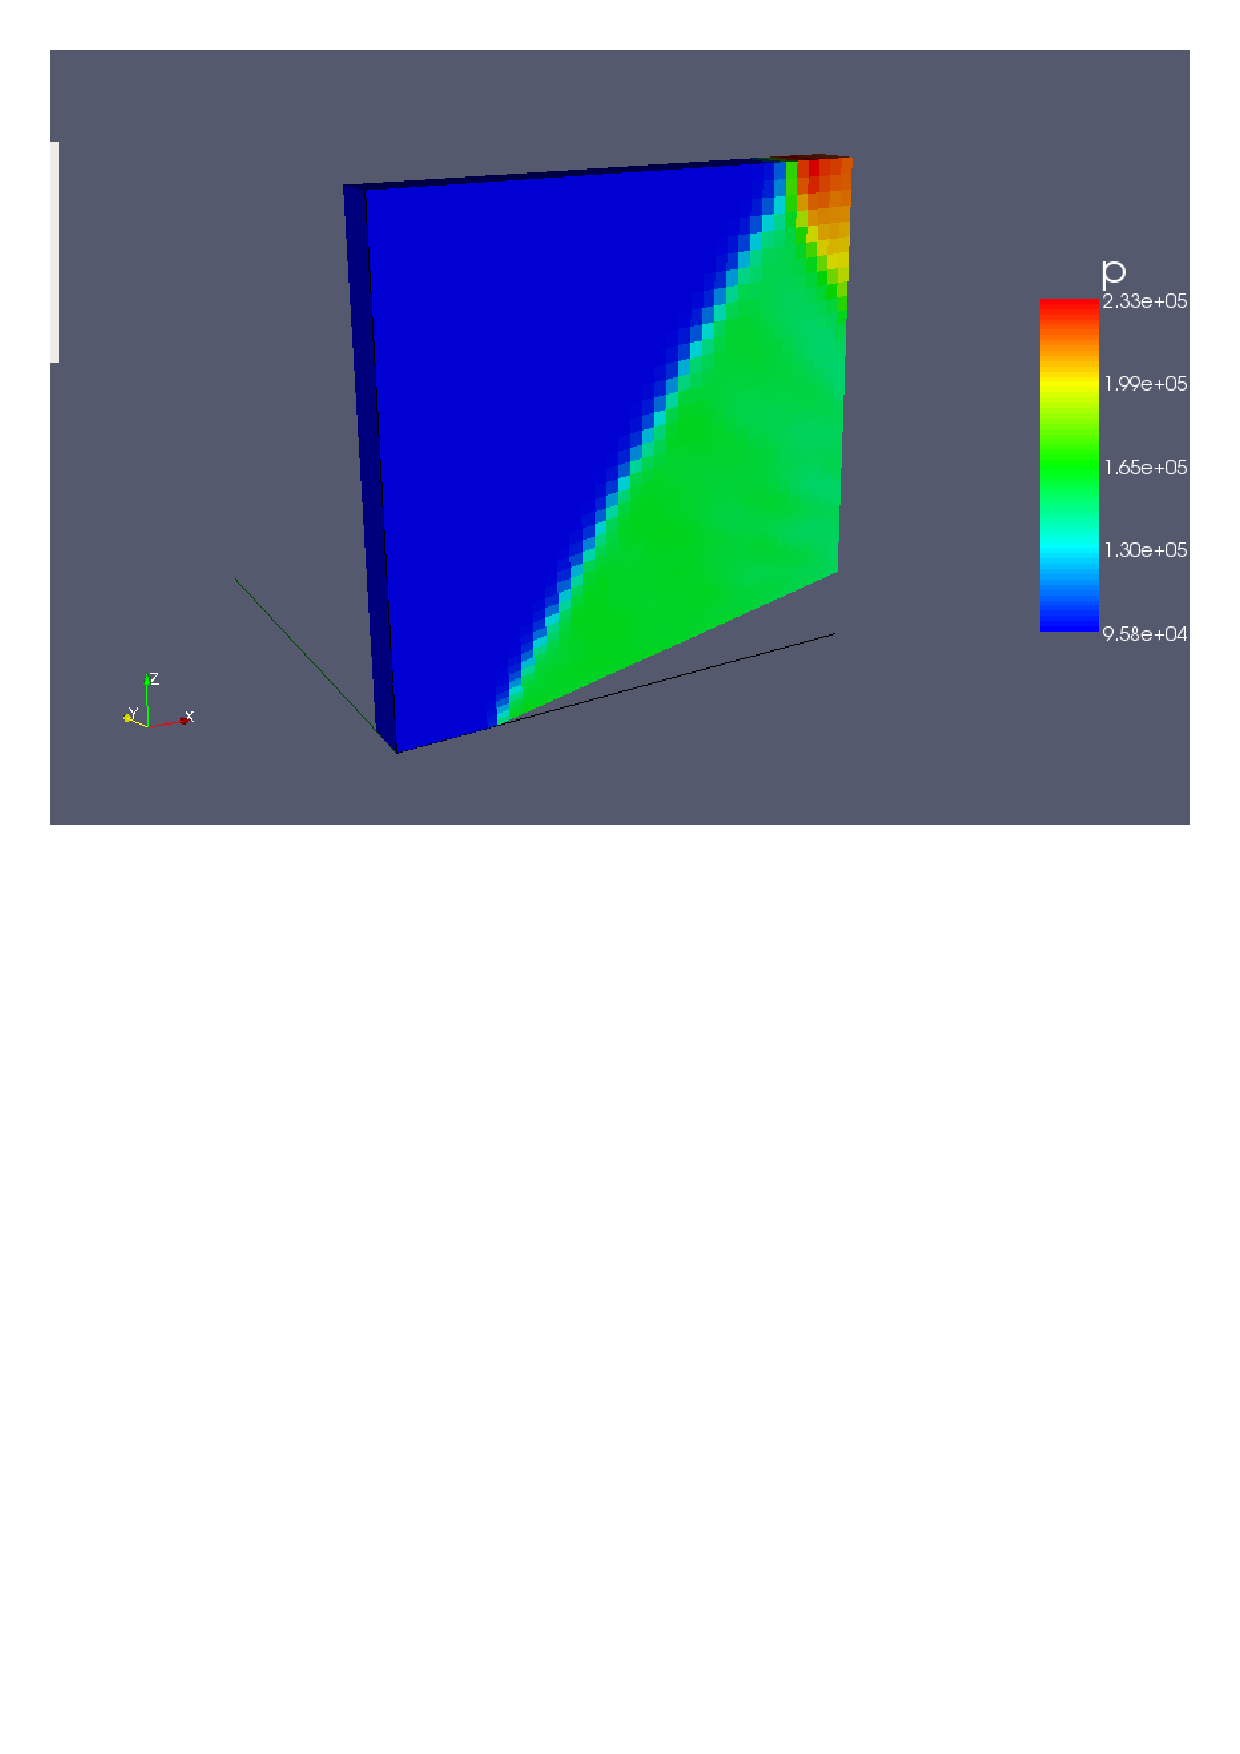
\includegraphics[width=10cm,viewport=27 444 571 818]{../3D/simple_ramp/simple-ramp-p.pdf}
\end{center}
\caption{Filled surface representation of the cells
  Colours representing pressure at $t = 5.0$\,ms.
  The 10$^o$ slope on the ramp is seen running up to the right.
  Note that the shock propagating from the start of the ramp is nearly
  straight until it approaches the top surface of the simulation domain where
  it is reflected.
  This PDF figure was generated with Paraview from the final solution file.}
\label{simple-ramp-p-fig}
\end{figure}

\begin{figure}[htbp]
\begin{center}
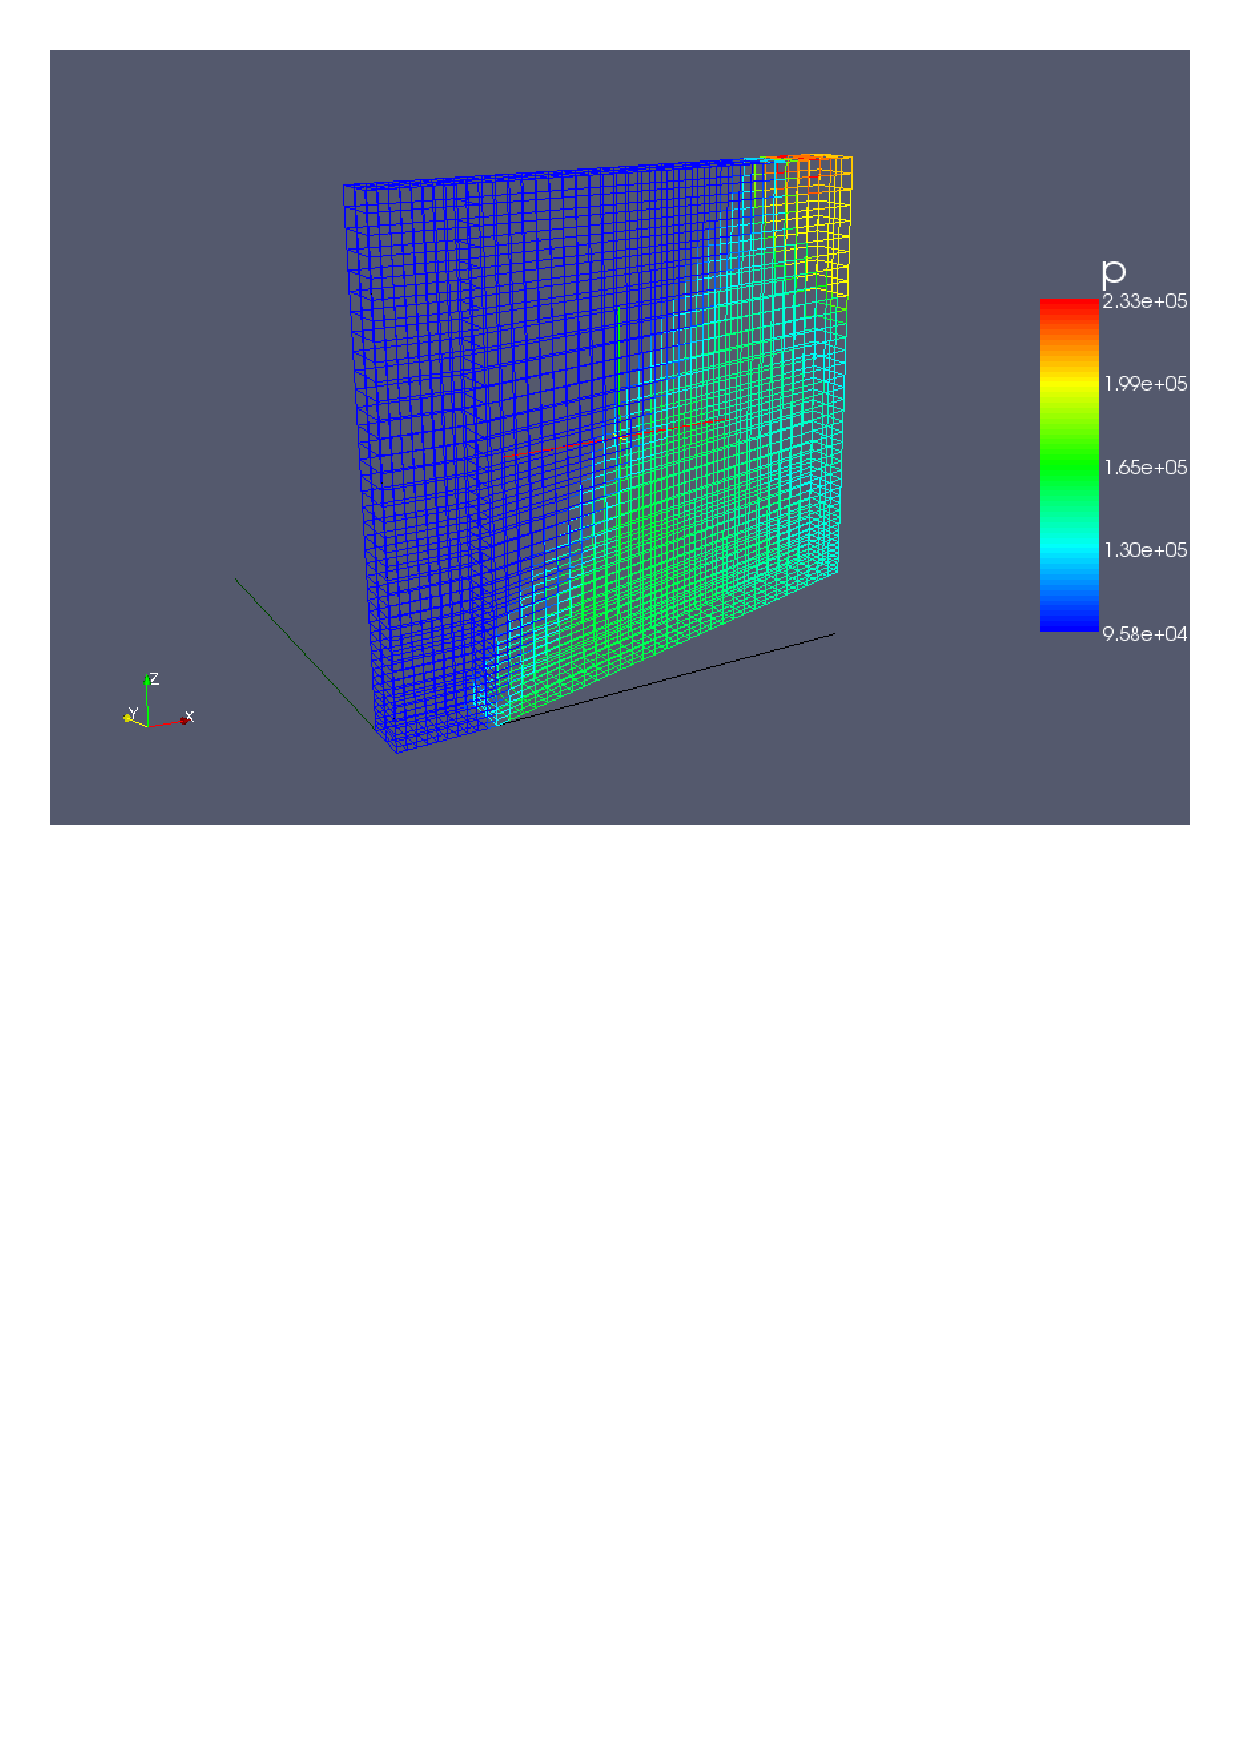
\includegraphics[width=10cm,viewport=27 444 571 818]{../3D/simple_ramp/simple-ramp-wire-frame-p.pdf}
\end{center}
\caption{Wireframe representation of the cells on the outer surfaces of the blocks.
  The grid is coloured, representing pressure at $t = 5.0$\,ms.}
\label{simple-ramp-wireframe-fig}
\end{figure}

\medskip
The postprocessing stage is the most variable part of the flow simulation
process.
Just what a user of the code wants to do in detail is often unclear at the
start of a simulation exercise but visualizing the data is usually the first
action in postprocessing.
Using the visualization software, ParaView\footnote{The Parallel Visualization
  Application (\url{http://www.paraview.org}) developed by Kitware
  (\url{http://www.kitware.com}) is freely available for download.},
one may view the transient development of the planar shock travelling over the
ramp and establishing the steady-flow oblique shock seen in
Fig.\,\ref{simple-ramp-p-fig}.
Starting with VTK parallel file \texttt{simple\_ramp.t0000.pvtu}, 
ParaView understands the time-stamp sequence
numbering of the VTK output files and allows you to step back and forth in
time and study the time development of the flow field.

\medskip
Visualization is often followed by a more quantitative analysis.  
The Python program in section\,\ref{simple-ramp-post-files}, for example,
picks up the data and computes the pressure force on the inclined surface of
the ramp.
The end result is \texttt{force= Vector3(2209.07, 0, -12528.2) Newtons}.
The \texttt{BlockGrid3D} class provides methods to read the grid and flow
solution for any particular block and makes the data available as a
multidimensional array.
The \texttt{libgeom2} module provides a number of geometric methods and these
are used to compute the cell interface properties on the surface of the ramp.
The final section of the postprocessing program computes the distances of the
cell centres from the ramp surface for a strip of cells along the ramp.
Such data might be useful when computing shear stress or heat flux, for example.


\subsection{Input script (.py)}
\topbar
\lstinputlisting[language={}]{../3D/simple_ramp/simple_ramp.py}
\bottombar


\subsection{Shell script}
\label{simple-ramp-sh-files}
\topbar
\lstinputlisting[language={}]{../3D/simple_ramp/simple_ramp_run.sh}
\bottombar


\subsection{Postprocessing program}
\label{simple-ramp-post-files}
\topbar
\lstinputlisting[language={}]{../3D/simple_ramp/estimate_ramp_force.py}
\bottombar

\subsection{Notes}
\begin{itemize}
\item None.
\end{itemize}
